
\begin{frame}{Where is Kotlin}
	\begin{columns}
		\begin{column}{0.5\textwidth}
			\onslide<2->{
				\begin{figure}
					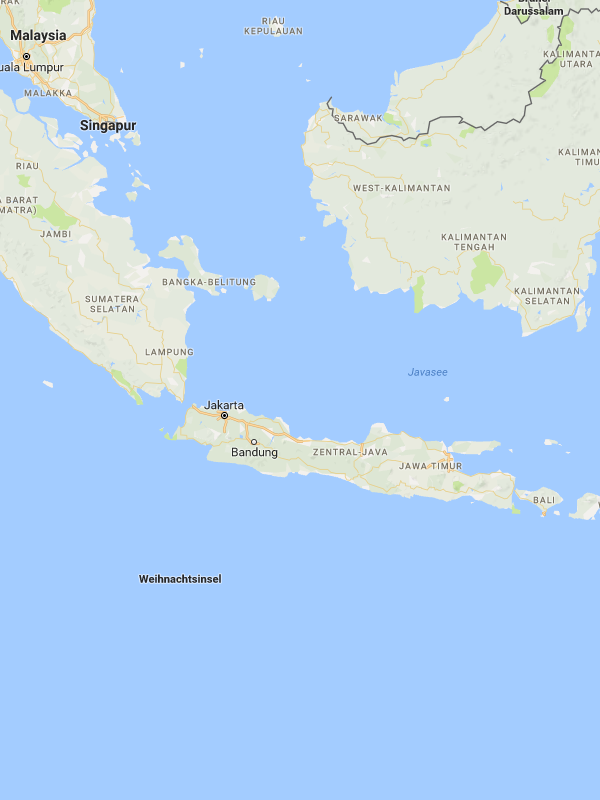
\includegraphics{figures/java}
					\caption{Java}
				\end{figure}
			}
		\end{column}
		\begin{column}{0.5\textwidth}
			\onslide<3->{
				\begin{figure}
					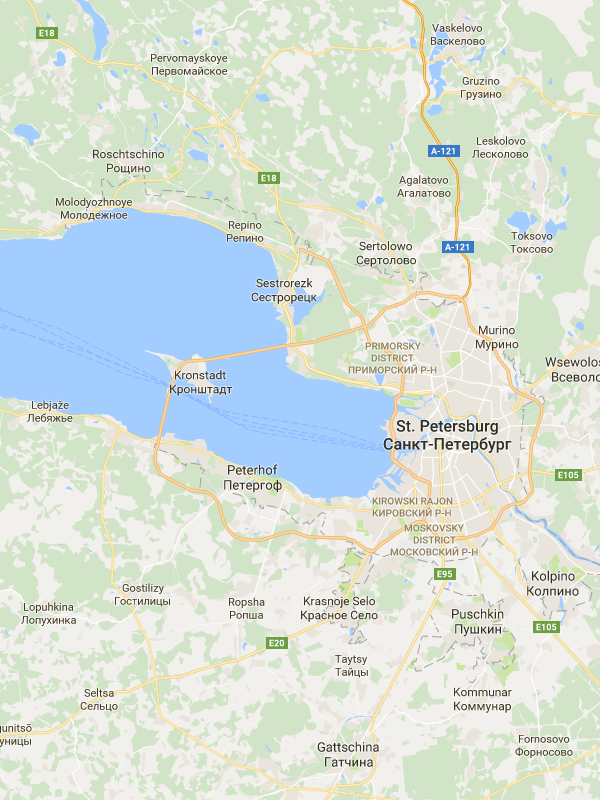
\includegraphics{figures/kotlin}
					\caption{Kotlin}
				\end{figure}
			}
		\end{column}
	\end{columns}
\end{frame}

\begin{frame}{What is Kotlin}
	\begin{itemize}
		\item JetBrains Project - Started 2010
		\item 1.0 Release in February 2016
		\item 1.1 Release in March 2017 (since June: 1.1.3)
		\item 1.2 M1 Release in June 2017
		\item JVM Language (JavaScript and Native in development)
		\item Fast ramp-up
		\item Easy tool-able
		\item Kotlin Standard Library
		\item Small footprint $\leq$ 1MB
		\item Non-Scientific borrow well-established patterns and concepts 
	\end{itemize}
\end{frame}

\begin{frame}{What is Kotlin}
	\begin{itemize}
		\item Java 6 compatible (mobile acceptance)
		\begin{itemize}
			\item Modern features 
		\end{itemize}
		\item Full backward compatibility in minor releases
		\begin{itemize}
			\item Easy and mostly automated migration paths for major releases 
		\end{itemize}
		\item Maven / Gradles support (including useful plugins)
		\begin{itemize}
			\item Kotlin language support for Gradle build scripts
		\end{itemize}
		\item Free Eclipse \& IntelliJ (community) integration
		\item Android support (official since Google I/O 2017)
		\item Spring Boot Kotlin extension (official in Spring 5)
	\end{itemize}
\end{frame}

\section{Key Concepts \& Features}

\begin{frame}{Key Concepts \& Features}
	\begin{itemize}
		\item easy mixing with Java (see samples) \cmark
		\item easy/short idiomatic access (var \& val, getter, setter, data) \cmark
		\item get rid of boilerplate code \cmark
		\item statically typed \cmark
		\item automatically inferred types \cmark
		\item default to closed instead of open classes (+sealed) \tmark
		\item classes \& objects \tmark
		\item nullable? (a billion dollar mistake !!) \cmark
		\item Pairs \& Triples \& Deconstructing \cmark
	\end{itemize}
\cmark \dots full sample, \tmark \dots partial sample, \xmark \dots no sample
\end{frame}


\begin{frame}{Key Concepts \& Features}
	\begin{itemize}
		\item default to Unit instead of Void as return type \xmark 
		\item lazy properties and delegations \cmark
		\item no checked exceptions \xmark
		\item functional programming (let it lamda) \tmark
		\item higher-order functions \tmark
		\item extension methods \cmark
		\item explicit module system \xmark
		\item runs on android \xmark
		\item can compile to JavaScript \xmark
	\end{itemize}
\cmark \dots full sample, \tmark \dots partial sample, \xmark \dots no sample
\end{frame}

\section{Code Samples}

\begin{frame}[fragile]{lst1}
\begin{lstlisting}[caption={Simple code listing.}, label={lst:example1}, language=Kotlin]
// this is a simple code listing:
println("hello kotlin from latex")
\end{lstlisting}
\end{frame}

\section{Traps \& Pitfalls}

\begin{frame}{Traps \& Pitfalls: Spring, Hibernate, \dots}
	\begin{itemize}
		\item Springs field injection does not work cause all fields are not null
		\begin{itemize}
			\item use "lateinit" on your @Autowired fields
			\item seriously use constructor injection over field injection
		\end{itemize}
		\item Classes are closed by default\\
		Spring can not proxy closed (final) classes
		\begin{itemize}
			\item use the "kotlin-allopen" maven/gradle plugin
			\item use the "kotlin-spring" maven/gradle plugin
		\end{itemize}
		\item Data classes have no non-argument constructor\\
		Hibernate/Jackson need non-argument constructor to create instances
		\begin{itemize}
			\item use the "kotlin-jpa" maven/gradle plugin
			\item use the "kotlin-noarg" maven/gradle plugin
		\end{itemize}
	\end{itemize}
\end{frame}

\begin{frame}[fragile]{Traps \& Pitfalls: Loopception}
	\begin{onlyenv}<1->
		\begin{lstlisting}[language=Kotlin]
fun loopception() {
	for(i in 1..2) {
		print("$i")
		for (j in 3..4) {
			print("$j")
			if (j== 3) break
}}}

fun main(args: Array<String>) = loopception()
		\end{lstlisting}
	\end{onlyenv}
	\begin{onlyenv}<2->
		\textbf{Outputs:} "1323"
	\end{onlyenv}
\end{frame}

\begin{frame}[fragile]{Traps \& Pitfalls: Loopception}
\begin{onlyenv}<1->
	\begin{lstlisting}[language=Kotlin]
fun loopception() {
	outerLoop@for(i in 1..2) {
		print("$i")
		for (j in 3..4) {
			print("$j")
			if (j== 3) break@outerLoop
}}}

fun main(args: Array<String>) = loopception()
	\end{lstlisting}
	\end{onlyenv}
	\begin{onlyenv}<2->
		\textbf{Outputs:} "13"\\\vspace{\baselineskip}
	\end{onlyenv}
	\begin{onlyenv}<3->
		\textbf{return} \dots returns from the nearest enclosing function\\
		\textbf{break} \dots terminates the nearest enclosing loop\\
		\textbf{continue} \dots proceeds to the next step of the nearest enclosing loop
	\end{onlyenv}
\end{frame}


\begin{frame}[fragile]{Traps \& Pitfalls: The return of power throw}
	\begin{onlyenv}<1->
		\begin{lstlisting}[language=Kotlin]
fun powerThrow() {
	return throw throw return
}

fun main(args: Array<String>) = powerThrow()
		\end{lstlisting}
	\end{onlyenv}
	\begin{onlyenv}<2->
		Yep it compiles\\
		return returns from the nearest enclosing function\\
		return itself returns type Unit()
	\end{onlyenv}
\end{frame}

\begin{frame}[fragile]{Traps \& Pitfalls: Almighty Type Inference}
	\begin{onlyenv}<1->
		\begin{lstlisting}[language=Kotlin]
fun hello() = print("Hello")
fun world() = {
	print(" World")
}

fun main(args: Array<String>) {
	hello()
	world()
}	
		\end{lstlisting}
	\end{onlyenv}
	\begin{onlyenv}<2->
		\textbf{Output:} "Hello"
	\end{onlyenv}
\end{frame}

\begin{frame}[fragile]{Traps \& Pitfalls: Almighty Type Inference}
	\begin{onlyenv}<1->
		\begin{lstlisting}[language=Kotlin]
fun hello(): Unit = print("Hello")
fun world(): () -> Unit = {
	print(" World")
}

fun main(args: Array<String>) {
	hello()
	world().invoke()
}
		\end{lstlisting}
	\end{onlyenv}
	\begin{onlyenv}<2->
		\textbf{Output:} "Hello World"
	\end{onlyenv}
\end{frame}

\section{Kotlin Native}

\begin{frame}[fragile]{Kotlin Native: GTK3}
	Check it out:\\
	\begin{lstlisting}[language=bash,basicstyle=\ttfamily\small]
mkdir kotlin-native-samples && \
cd kotlin-native-samples && \
git init && \
git config core.sparseCheckout true && \
git remote add -f origin \
	https://github.com/JetBrains/kotlin-native.git && \
echo "samples/*" > .git/info/sparse-checkout && \
git checkout v0.3
	\end{lstlisting}
\end{frame}

\begin{frame}[fragile]{Kotlin Native: GTK3}
	Compile your first sample:\\
	\begin{lstlisting}[language=bash,basicstyle=\ttfamily\small]
docker run --rm -ti --workdir /sample -u root \
-v "$(pwd)/samples/gtk:/sample" \
hemeroc/kotlin-native:v0.3.0 \
/bin/bash -c \
"apt-get update; apt-get install libgtk-3-dev; ./build.sh"
	\end{lstlisting}
	Try it out\\
	\begin{lstlisting}[language=bash,basicstyle=\ttfamily\small]
./samples/gtk/build/bin/Gtk3Demo.kexe
	\end{lstlisting}
\end{frame}

\begin{frame}[fragile]{Kotlin Native: GTK3}
	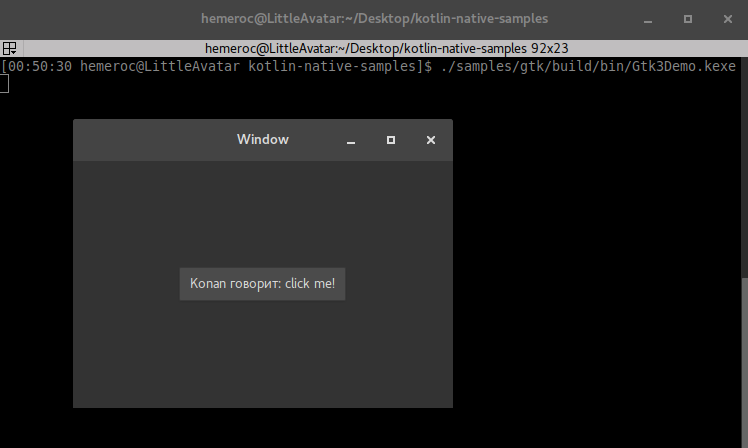
\includegraphics[width=0.85\paperwidth]{figures/gtk3}
\end{frame}

\section{Contribute \& Get Started}

{
\usebackgroundtemplate{\parbox[c][\paperheight][c]{\paperwidth}{\centering\transparent{0.1}
\includegraphics[width=1\paperwidth]{figures/kotlinLogo1}}
}%

\begin{frame}{Contribute}
	\vspace*{\stretch{1}}%
	\begin{center}
		\LARGE \href{https://youtrack.jetbrains.com/issues/KT/}{https://youtrack.jetbrains.com/issues/KT/}\\
		\href{https://github.com/Kotlin/KEEP}{https://github.com/Kotlin/KEEP}
	\end{center}
	\vspace*{\stretch{1}}%
\end{frame}

\begin{frame}{Getting Started}
	\vspace*{\stretch{1}}%
	\begin{center}
		\LARGE \href{https://kotlin.link/}{https://kotlin.link/}\\
		\href{http://slack.kotlinlang.org/}{http://slack.kotlinlang.org/}\\
		\href{https://github.com/Kotlin/kotlin-koans}{https://github.com/Kotlin/kotlin-koans}
	\end{center}
	\vspace*{\stretch{1}}%
\end{frame}
}

\begin{frame}{Thank You}
	\vspace*{\stretch{1}}%
	\begin{center}
		\LARGE Get started with\\
		\vspace{.5cm}
		{\transparent{1}
\includegraphics[width=.5\paperwidth]{figures/kotlinLogo2}}\\
		\vspace{.5cm}
		\href{https://try.kotlinlang.org/}{https://try.kotlinlang.org/}
	\end{center}
	\vspace*{\stretch{1}}%
\end{frame}